\documentclass[working]{tuftebook}
\usepackage[utf8]{inputenc}
\usepackage[T1]{fontenc}
\usepackage{textcomp}

\usepackage{url}

\usepackage{biblatex}
\addbibresource{bibliography.bib}

\usepackage{hyperref}
\hypersetup{
    colorlinks,
    linkcolor={black},
    citecolor={black},
    urlcolor={blue!80!black}
}
\usepackage[noabbrev]{cleveref}

% Adds Bibliography, ... to Table of Contents
\usepackage[nottoc]{tocbibind}

\usepackage{graphicx}
\usepackage{float}
\usepackage[usenames,dvipsnames,svgnames]{xcolor}

% \usepackage{cmbright}

\usepackage{amsmath, amsfonts, mathtools, amsthm, amssymb}
\usepackage{mathrsfs}
\usepackage{cancel}

\newcommand\N{\ensuremath{\mathbb{N}}}
\newcommand\R{\ensuremath{\mathbb{R}}}
\newcommand\Z{\ensuremath{\mathbb{Z}}}
\renewcommand\O{\ensuremath{\emptyset}}
\newcommand\Q{\ensuremath{\mathbb{Q}}}
\newcommand\C{\ensuremath{\mathbb{C}}}
\let\implies\Rightarrow
\let\impliedby\Leftarrow
\let\iff\Leftrightarrow
\let\epsilon\varepsilon

\usepackage{tikz}
\usepackage{tikz-cd}

% theorems
\usepackage{thmtools}
\usepackage[framemethod=TikZ]{mdframed}
\mdfsetup{skipabove=1em,skipbelow=0em, innertopmargin=12pt, innerbottommargin=8pt}

\theoremstyle{definition}

\makeatletter

\declaretheoremstyle[headfont=\bfseries\sffamily, bodyfont=\normalfont, mdframed={ nobreak } ]{thmgreenbox}
\declaretheoremstyle[headfont=\bfseries\sffamily, bodyfont=\normalfont, mdframed={ nobreak } ]{thmredbox}
\declaretheoremstyle[headfont=\bfseries\sffamily, bodyfont=\normalfont]{thmbluebox}
\declaretheoremstyle[headfont=\bfseries\sffamily, bodyfont=\normalfont]{thmblueline}
\declaretheoremstyle[headfont=\bfseries\sffamily, bodyfont=\normalfont, numbered=no, mdframed={ rightline=false, topline=false, bottomline=false, }, qed=\qedsymbol ]{thmproofbox}
\declaretheoremstyle[headfont=\bfseries\sffamily, bodyfont=\normalfont, numbered=no, mdframed={ nobreak, rightline=false, topline=false, bottomline=false } ]{thmexplanationbox}

\declaretheoremstyle[headfont=\bfseries\sffamily, bodyfont=\normalfont, numbered=no, mdframed={ nobreak, rightline=false, topline=false, bottomline=false } ]{thmexplanationbox}


\declaretheorem[numberwithin=chapter, style=thmgreenbox, name=Definition]{definition}
\declaretheorem[sibling=definition, style=thmredbox, name=Corollary]{corollary}
\declaretheorem[sibling=definition, style=thmredbox, name=Proposition]{prop}
\declaretheorem[sibling=definition, style=thmredbox, name=Theorem]{theorem}
\declaretheorem[sibling=definition, style=thmredbox, name=Lemma]{lemma}
\declaretheorem[sibling=definition, style=thmbluebox,  name=Example]{eg}
\declaretheorem[sibling=definition, style=thmbluebox,  name=Nonexample]{noneg}
\declaretheorem[sibling=definition, style=thmblueline, name=Remark]{remark}




\declaretheorem[numbered=no, style=thmexplanationbox, name=Proof]{explanation}
\declaretheorem[numbered=no, style=thmproofbox, name=Proof]{replacementproof}
\declaretheorem[style=thmredbox,  numbered=no, name=Exercise]{ex}
\declaretheorem[style=thmblueline, numbered=no, name=Note]{note}

% \renewenvironment{proof}[1][\proofname]{\begin{replacementproof}}{\end{replacementproof}}

% \AtEndEnvironment{eg}{\null\hfill$\diamond$}%

\newtheorem*{uovt}{UOVT}
\newtheorem*{notation}{Notation}
\newtheorem*{previouslyseen}{As previously seen}
\newtheorem*{problem}{Problem}
\newtheorem*{observe}{Observe}
\newtheorem*{property}{Property}
\newtheorem*{intuition}{Intuition}


\declaretheoremstyle[
    headfont=\bfseries\sffamily\color{RawSienna!70!black}, bodyfont=\normalfont,
    mdframed={
        linewidth=2pt,
        rightline=false, topline=false, bottomline=false,
        linecolor=RawSienna, backgroundcolor=RawSienna!5,
    }
]{todo}
\declaretheorem[numbered=no, style=todo, name=TODO]{TODO}


\usepackage{etoolbox}
\AtEndEnvironment{vb}{\null\hfill$\diamond$}%
\AtEndEnvironment{intermezzo}{\null\hfill$\diamond$}%

% http://tex.stackexchange.com/questions/22119/how-can-i-change-the-spacing-before-theorems-with-amsthm
% \def\thm@space@setup{%
%   \thm@preskip=\parskip \thm@postskip=0pt
% }

\usepackage{xifthen}

\makeatother

% figure support (https://castel.dev/post/lecture-notes-2)
\usepackage{import}
\usepackage{xifthen}
\pdfminorversion=7
\usepackage{pdfpages}
\usepackage{transparent}


\makeatletter
\newif\ifworking
\@ifclasswith{tuftebook}{working}{\workingtrue}{\workingfalse}
\makeatother

\newcommand{\incfig}[2][1]{%
    % \ifworking{\makebox[0pt][c]{\color{gray}{\scriptsize\textsf{#2}}}}\fi%
    \def\svgwidth{#1\textwidth}
    \import{./figures/}{#2.pdf_tex}
}

\newcommand{\fullwidthincfig}[2][0.90]{%
    % \ifworking{\makebox[0pt][l]{\color{gray}{\scriptsize\textsf{#2}}}}\fi%
    \def\svgwidth{#1\paperwidth}
    \import{./figures/}{#2.pdf_tex}
}



\newcommand{\minifig}[2]{%
    \def\svgwidth{#1}%
    \begingroup%
    \setbox0=\hbox{\import{./figures/}{#2.pdf_tex}}%
    \parbox{\wd0}{\box0}\endgroup%
}

% %http://tex.stackexchange.com/questions/76273/multiple-pdfs-with-page-group-included-in-a-single-page-warning
\pdfsuppresswarningpagegroup=1

\newcommand\todo[1]{\ifworking {{\color{red}{#1}}} \else {}\fi}

\author{Gilles Castel}

\usepackage{pdfpages}

\usepackage{lipsum}
\usepackage{parskip}
\usepackage{titletoc}

\usepackage{cmbright}
\usepackage{bm}

\title{Rapport - Read-out Noise, Dark Charge og Signal to Noise Ratio i Princeton Instruments CCD-kamera.}
\author{Albert Lunde, Tinus Blæsbjerg}
\date{Academic year 2020--2021}

\begin{document}    
\renewcommand{\thepage}{\roman{page}}

\includepdf[pages=-, fitpaper=true]{./frontmatter.pdf}
\pagestyle{fancy}

\begingroup
\let\cleardoublepage\relax
\let\clearpage\relax  
\maketitle
\endgroup


\begingroup
\let\cleardoublepage\relax
\let\clearpage\relax  
\tableofcontents
\endgroup
\let\cleardoublepage\clearpage
\chapter{Problemformulering}
Vi vil i denne rapport undersøge billeder taget af et CCD Camera fra Princeton Instruments, med henblik på at bestemme kameraets read-out-noise til forskellige indstillinger. I forlængelse af dette, vil vi kigge på, hvordan forholdet er mellem de forskellige read-out-noises, og den usikkerhed der forbundet med den målte poissonfordelte data. Dette vil vi så bruge til at vurdere kameraets kvalitet. Hvis vi bliver færdig med overstående i god tid, vil vi også kigge på, hvordan dark charge giver anledning til mere støj.

\chapter{Teori}
I denne del beskriver vi teorien bag \textbf{read-out noise}, \textbf{dark charge} og \textbf{signal to noise ratio}. Vi beskriver desuden de statistiske metoder vi har brugt til at beregne usikkerheden på disse størrelser.
\section{Read-out Noise}
\begin{marginfigure}
    \centering
    \incfig{read-out-noise}
    \caption{Read-out-noise: Hver pixel læses lineært af kameraet. Først tømmes øverste række, derefter rykkes næste kollonne op.}
    \label{fig:read-out-noise}
\end{marginfigure}
Et CCD er opbygget af et gitterværk af elektriske brønde. Hver af brøndene svarer til én pixel på det endelige billede som kameraet giver. Når én af disse brønde rammes af en foton, omdanner brønden denne foton til elektrisk ladning. Desto flere ladninger der rammer brønden des større ladning. Når shutteren i kameraet lukkes, oversætter den nu disse ladninger i brøndene til en lysstyrke svarende til størrelsen af ladningen. Støjen kommer rent mekanisk fra designet af kameraet, hvor 

\subsection{Hvad er Read-out Noise?}
Hvad er read-out noise konkret? Ideelt set, så burde to billeder taget med de samme indstillinger være identiske, men dette er ikke tilfældet, hvilket man ville kunne se, hvis man sammenlignede en masse billeder med hinanden. Denne variation i billederne er essensen af read-out-noise, fordi hvis der ingen støj var, så ville billederne netop være ens. Så hvis man estimere denne usikkerhed, så kan man fraregne den fra ens faktisk data, og på den måde få bedre data. 
\\
Hvordan beskriver vi denne støj? Man kan ikke estimere den udfra et billede, men hvis vi har to billeder, som vi kan sammenligne, så kan vi finde ud af, hvad differencen mellem de to billeder er, hvilket vi kan bruge til at estimere, hvad støjen på et billede er. Det skyldes, at når vi kigger på differencen mellem de to billeder, så propagerer vi fejlen fra de enkelte billeder gennem en multivariabel funktion, som vi godt kan finde fejlen på. 
Dette kan fx gøres ved at bruge den calculus-baseret approksimation for en multi-variabel funktion. Funktionen er givet ved:
\[
Z = A - B
.\] 
Fejlen estimeres vha. følgende udtryk:
\begin{align*}
	(\alpha_Z)^2&=\left|   \frac{\partial Z}{\partial A}\right|^2(\alpha_A)^2+\left|   \frac{\partial Z}{\partial B}\right|^2(\alpha_B)^2 \\
	\alpha_Z&=\sqrt{(\alpha_A)^2+(\alpha_B)^2}
.\end{align*}
Fejlen på Z kan nemt beregnes i praksis, fordi man har en masse datapunkter, som man kan finde både middelværdi og spredningen på.
\\
Fejlen på A og B må nødvendigvis være den samme, da de pga samme kameraindstillinger , må komme fra den samme statistiske fordeling. Derfor kan man omskrive udtrykket:
\begin{align*}	
	\alpha_Z&=\sqrt{2(\alpha_A)^2} \\
	\alpha_Z&=\sqrt{2}\cdot \alpha_A \\
	\alpha_A&=\frac{\alpha_Z}{\sqrt{2}}
.\end{align*}

Read-out noise er jo netop den flukturation omkring hvert datapunkt, der gør, at det samme datapunkt på to seperate billeder kan have forskellige værdier. Så et godt estimat for denne støj, vil være spredningen omkring hvert datapunkt. Vi har vist at denne spredning kan findes, hvis man kigger på fejlen i Z. Men fejlen i Z stammer jo også fra den tilfældige flukturation associeret ved støjen af to billeder, derfor er spredningen af Z netop også et godt estimat for fejlen på Z. Med disse antagelser kan vi omskrive udtrykket fra før:
\begin{align*}
	noise&=\frac{\sigma_{Z}}{\sqrt{2}} 
.\end{align*}

Pr. konstruktion af forsøget er der taget 10 billeder med hver indstilling, hvilket betyder, at man kan tage differencen parvis for alle kombinationer af de 10 billeder. Dette giver en masse middelværdier for read-out noise, som vi kan tage middelværdien, for at få et godt estimat af hvad den faktiske read-out noise for et sæt af specifikke indstillinger er. Vi ved, at når vi tager middelværdien af noget data, så er der en usikkerhed forbundet med denne middelværdi, som er givet ved:
\begin{align*}
\alpha = \frac{\sigma_{N-1}}{\sqrt{N}}
\bar{x}\pm \alpha
.\end{align*}
\section{Plotning af data}
Efter vi har beregnet vores read-out noise til forskellige indstillinger, så skal vi også have tolket på vores data. Den bedste måde at gøre dette på, er selvfølgelig ved at plotte dataet. 

\subsection{Enkelte indstillinger}
Vi har gjort os en række overvejelser i forbindelse med plotningen af vores data, fordi vi skal have repræsenteret vores data på en overskuelig måde. Vi kom frem til, at vi gerne ville undersøge, hvordan de enkelte indstillinger påvirker den read-out noise man får ud. Måden vi har valgt at gøre det på, er ved at lave fire forskellige plots, hvor vi i hvert plot undersøger en bestemt indstilling. 
\\
\begin{marginfigure}[-100pt]
    \centering
    \incfig{bins}
    \caption{Kameraet kan indstilles til at udlæse pixels i \textbf{bins}, de mulige indstillinger er vist på figuren; 1x1, 4x4, 8x8 og 20x20. }
    \label{fig:bins}
\end{marginfigure}
Et eksempel kunne fx være \textbf{bin-indstillingen}, hvor man gerne vil undersøge, hvad der sker,når man ændrer på bin størrelsen. rent plotteteknisk gøres dette ved at sortere dataet i en bestemt rækkefølge på forhånd uafhængigt af bin indstillingen. Det betyder, at punkterne med identiske indstillinger på nær bin indstillingen kommer til at ligge over hinanden i plottet. Derefter kan man så farvekode de forskellige bin indstillinger, så man nemt kan se, hvordan ændringen i bins ændrer ens read-out-noise. Dette kan gøres ved alle indstillinger.
\subsection{Bedste indstilling}
Udover at kigge på, hvordan de enkelte indstillinger påvirker read-out noisen, så  vil vi også kigge på alle indstillingerne i et samlet plot. Her vil vi prøve at finde frem til, hvilket sæt af indstillinger, der giver den laveste read-out noise.
\subsection{Fit og fejlpropagering}
De steder i rapporten hvor vi har fittet vores data til funktioner, har vi lavet lavet fejlpropagering på fittet. Vi har brugt ophobningsloven via. den funktionelle metode. Med hjælp af den funktionelle udregnes fejlen på hvert punkt til at være,
\begin{align*}
	\alpha _z^2= &\left[ f\left( A + \alpha_A, B, C, \ldots \right) - f\left( A, B, C, \ldots\right)   \right]^2  \\
	 + &\left[ f\left( A, B + \alpha _B, C, \ldots  \right) - f\left( A, B, C, \ldots\right)   \right]^2 \\
	 + &\left[ f\left( A, B, C+\alpha_C , \ldots  \right) - f\left( A, B, C, \ldots\right)   \right]^2\\
	 + & \ldots
\end{align*}
I tilfældet hvor funktionen tager tiden $t$ som en parameter, antager vi at usikkerheden på $t$ er neglicibel. På vores har vi skraveret usikkerheden omkring fittet. I de fleste tilfælde har usikkerheden på fittet dog været så lille at det skraverede areal ikke kan ses på plottet.
\section{Dark Noise}
En anden støj som vi også kan kigge på, er den støj som er forbundet med \textbf{dark current}.
\begin{marginfigure}
	\textbf{Dark current:} Elektroner genereres spontant inde i kameraet, hvilket resulterer i en strøm, når man kigger på et tidsinterval og deraf navnet. Den spontane generering af elektroner er stærkt temperaturafhængig, så hvis kameraet køles, reduceres denne strøm meget.\cite{HH}

\end{marginfigure}
Ved alle målinger med kameraet, hvor man observerer i et tidsrum, vil der være dark current tilstede i ens data. Så i princippet, når man udlæser ens data fra kammeraet, vil en lille del af det signal man måler kommer fra de termisk genererede elektroner. I princippet kan man jo så tage en baggrundsmålling, inden man går videre til det rigtige forsøg. Denne måling kan man så tage højde for, når man laver sine faktiske målinger og på den måde tilnærmelsesvis eliminere bidraget fra dark current. Man vil så ikke helt få elimineret bidraget fra dark current, fordi der er en støj forbundet med denne, heraf \textit{dark noise}. Denne støj kommer af, at dark current afhænger af antal elektroner der er talt. Det betyder, at det er poisson fordelt. 
\\
Når noget er poissonfordelt, så ved vi, at fejlen er givet ved \sidenote{Measurements and uncertenties side 30}:
\begin{align*}
\alpha = \sqrt{N} \\
\end{align*}
Det vil sige, at på samme måde som read-out noise, så ville man måle en forskellig dark current, hvis man foretog den samme måling flere gange. 
\\
Vi ved at dark current er temperaturafhængig, hvilket også betyder, at dark noise er temperaturafhængig. Undersøgelser, som ligger uden for målet for denne opgave, viser at hvis man køler kameraet tilstrækkeligt, så er der næsten ikke noget bidrag fra dark noise. Det viser sig, at der er et lineært forhold mellem eksponeringstiden og antal af termisk generede elektroner, hvis temperaturen er konstant. Hvilket måske skal plottes? Plot også dark current med fejl
\subsection{Sammenligning af dark noise og read-out noise}
Vi kan prøve at lave en sammelinging af, hvilken en af de to faktorer, der bidrager mest til den totalle fejl på ens målte data. Vi ved fra bogen \sidenote{Measurements and uncertainties side 41} at: 
\begin{align*}
(\alpha_Z)^2 =(\alpha_Z^A)^2+(\alpha_Z^B)^2 + ...
\end{align*}
Hvilket i vores opgave vil svare til:
\begin{align*}
\alpha_{total} = \sqrt{\alpha_{d-noise}^2 + \alpha_{ro-noise}^2}. 
\end{align*}
I vores sammenligining, har vi plottet de 2 former for støj. Vi har underøgt til hvilken tid dark noise bliver større end read-out noise. Altså for hvilket $t'$ der gælder,
\[
	\alpha _{d} \left( t' \right)  - \alpha _{ro} = 0
.\]
For at bestemme usikkerheden $\alpha _{t'}$ på denne tid har vi gjort brug af ophobningsloven. Read-out noise er konstant over tid, mens Dark Noise er givet ved følgende udtryk,
\[
\alpha _d \left( t \right) = \sqrt{I_{dc}\cdot t} 
.\]
Usikkerheden på dark noise til tiden $t$, bestemmes ved at betragte funktionen,
\[
Z = \sqrt{I_{dc}\cdot t} 
.\] 
Vi kender $\alpha _{dc}$ og kan dermed bestemme $\alpha _Z$,
\begin{align*}
	\alpha_{z}^2 &= \left| \frac{\partial Z}{\partial I_{dc}} \right|^2\alpha_{dc}^2 = t^2 \cdot \left( \frac{1}{2\cdot \sqrt{I\cdot t} } \right)^2\cdot \alpha _{dc}^2 = \left( \frac{\sqrt{t}}{ 2\cdot \sqrt{I}} \right)^2 \cdot \alpha _{dc}^2 \\
	\alpha _z &= \left( \frac{\sqrt{t} }{2\cdot \sqrt{I} } \right) \cdot \alpha _{dc}
.\end{align*}
For at bestemme usikkerheden på skæringstiden $t'$, betragter vi nu funktionen,
 \[
Z'\left( t \right) = \sqrt{I_{dc}\cdot t} - RO
.\] 
Pr. ophobingsloven er usikkerden på $Z'$,
 \[
\alpha _Z'\left( t \right)  = \sqrt{\left( \frac{\sqrt{t} }{2\cdot \sqrt{I} } \right)^2 + \alpha _{ro}^2 }
.\]
Vi bestemmer altså først $t'$ ved at finde skæringspunktet mellem de 2 kurver. Vi bruger derefter funktionen $\alpha _Z'\left( t \right) $ til at bestemme usikkerheden på denne tid. \\
Det viser sig, at dark noise ikke bidrager specielt meget til den totale støj i forhold til read-out noise, men dette vil vi undersøge dybbere nede i resultaterne.

\subsection{Beregning af Dark Charge}
I vores undersøgelse af CCD-kameraet, har vi gjort brug af diverse metoder til at bestemme mængden af Dark Charge på et enkelt billede. Vi har fået givet 10 billeder taget til en bestemt tid $t$. For hvert af disse billeder har vi bestemt en gennemsnitlig pixel-lysstyrke $\overline{x}_i$ med en associeret usikkerhed $\alpha_i $. Disse middelværdier og usikkerheder er bestemt med samme metode som i \textbf{0.0.1}. Vi har derefter fundet den vægtede middelværdi af pixel-lysstyrken på tværs af de 10 billeder. Denne beregnes via\sidenote{HH ligning (4.30)},
\[
	\overline{x}_w = \frac{\sum_i w_i\overline{x}_i}{\sum_i w_i} 
,\]
hvor vægten $w_i$, er givet som\sidenote{HH ligning (4.31)}
 \[
w_i = \frac{1}{\alpha _i^2}
.\]
Usikkerheden på den vægtede middelværdi er givet som,
\[
\alpha_w =\left( \sum_{i} \frac{1}{\alpha _i^2}   \right)^{-2}
.\]
Pga. Dark Charges natur vil vores forventning være at størrelsen $\overline{x}_w$ vokser lineært med tiden. Vi har derfor fittet funktionen,
\[
\overline{x}_w\left( t \right)  = a\cdot t + b
.\]
til vores data og estimeret parametrene $a$ og $b$. Denne hældning $a$ vil være afhængig af bin-størrelsen, da en større bin , vil give anledning til et større areal hvorpå der kan dannes dark-charge. For at finde den faktiske dark-charge hældning deler vi derfor med arealet af binnet.
\[
a = \frac{a_b}{A_b}
.\] 
\section{Vurdering af kamera}
\chapter{Resulater}
\section{Read-out Noise}
Her følger plots af de forskellige indstillinger. Vi har valgt at samle de forskellige parametre i hver deres plot og dermed undersøge den overordnede som disse parametre har på read-out noise.
Et eksempel kunne fx være \textbf{bin-indstillingen}, hvor man gerne vil undersøge, hvad der sker, når man ændrer på bin-størrelsen. Rent plotteteknisk gøres dette ved at sortere dataet i en bestemt rækkefølge på forhånd uafhængigt af bin-indstillinge. Det betyder, at punkterne med identiske indstillinger på nær bin-indstillingen kommer til at ligge over hinanden i plottet. Derefter kan man så farvekode de forskellige bin-indstillinger, så man nemt kan se, hvordan ændringen i bins ændrer ens read-out noise. Dette kan gøres ved alle indstillinger.
\subsection{Bin-Indstilling}
\begin{figure}[ht]
\centering
\sidecaption{Plot af bins}
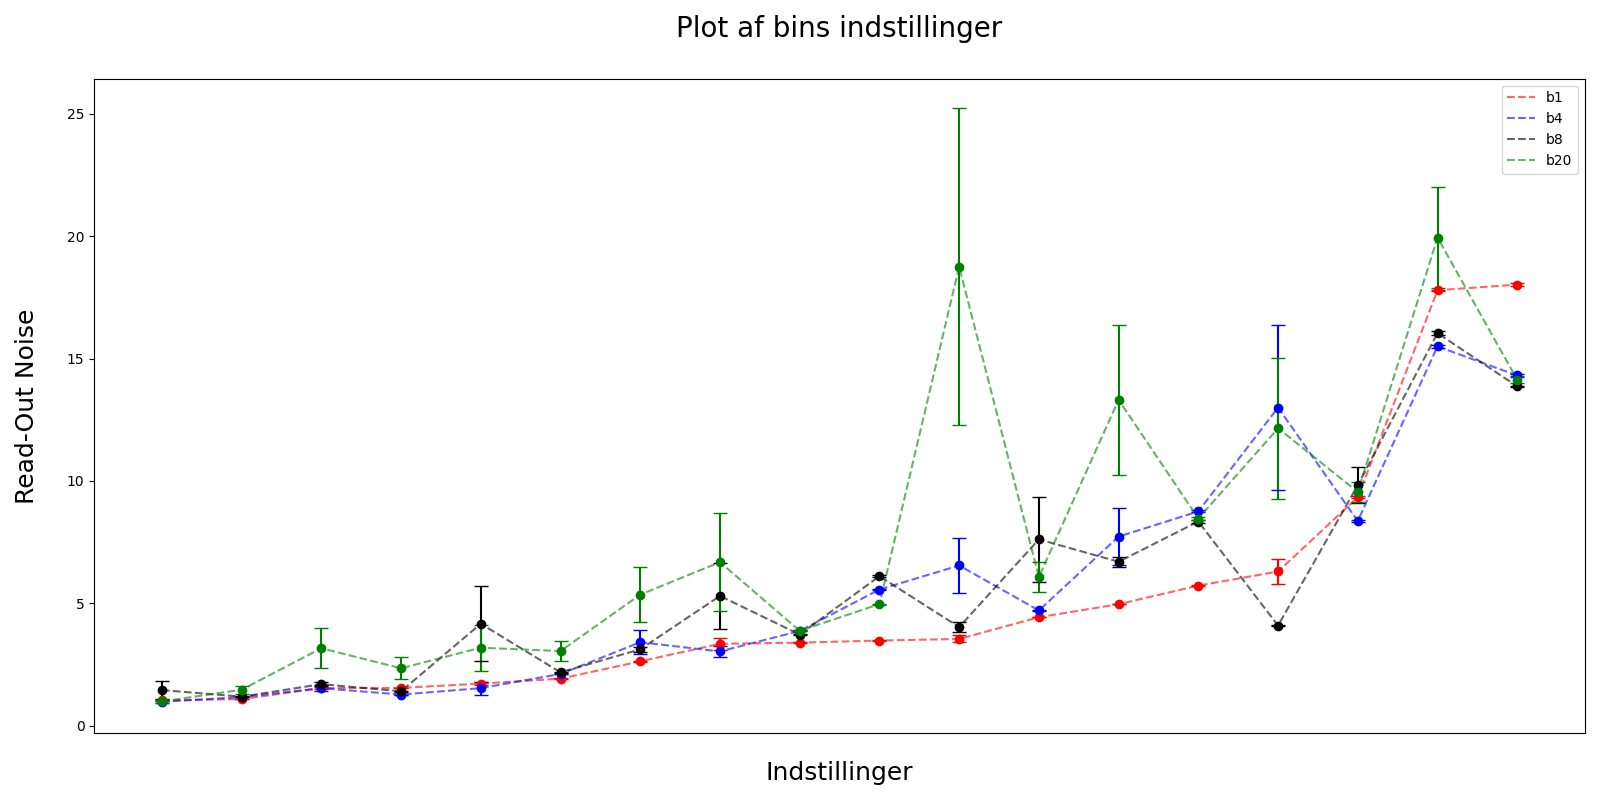
\includegraphics[width = \textwidth]{Plots/bins.png}	
\end{figure}
Hvis vi kigger på de røde punkter med bin-indstilling 1x1, så kan vi se, at den generelt har den laveste read-out noise over de fleste indstillinger, udover et par enkelte punkter til sidst. Men en ting man kan bide mærke i, når man kigger på de røde punkter er, at der ikke er en specielt stor fejl på værdierne. Det giver meget god meningen, fordi bin-indstillingen indvirker netop på hvor mange datapunkter der er i hvert billede. Hvis man har et højt antal datapunkter bliver ens måling mere præcis, hvilket betyder at hvert værdien af hvert datapunkt ikke flukturerer lige så meget som højrere bin-indstillinger. Hvis man så fx kigger på 20x20-indstillingen, så er der langt færre datapunkter, hvilket vil sige, at hvert datapunkt indeholder mere information. Det betyder også, at ens data bliver mere upræcis, hvilket så netop både giver anledning til en større read-out noise, men også større fejl på read-out noisen. Værdien for et datapunkt fluktuerer netop pga. af read-out noise, hvis man så har mange punkter indeholdende mindre information, så er flukturationen ikke nær så stor som et mindre antal punkter, ind
\subsection{Quality-Indstilling}
På quality-indstillingen ser vi at 'high-quality' næsten altid giver anledning til en lavere read-out noise end 'low-quality'. 'High-quality' giver desuden også en lavere usikkerhed på read-out noise.
\begin{figure}[ht]
\centering
\sidecaption{Plot af quality}
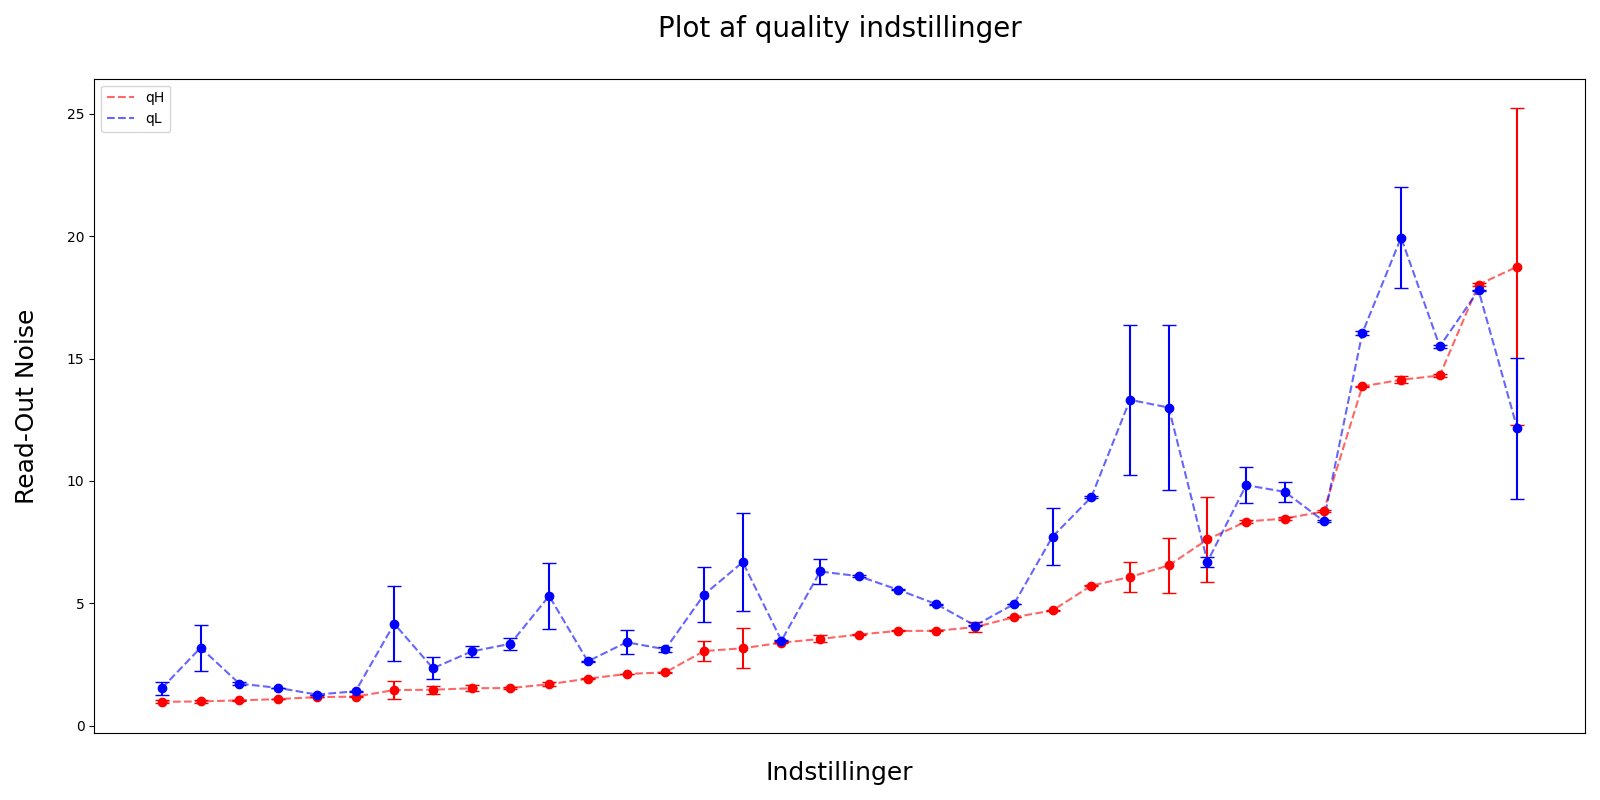
\includegraphics[width = \textwidth]{../Plots/quality.png}	
\end{figure}

\subsection{Gain-Indstilling} 
Ved 'gain' indstillingen ser vi følgende forhold som er overholdt på tværs af stort set alle indstillinger,
\[
gH > gM < gL
.\]
Dette giver god mening da gain er et mål for hvor forholdt strøm målt i en bin og lysstyrken på pixelen denne oversættes til. En høj gain vil dermed betyde at der skal færre elektroner til at skabe en høj lysstyrke på billedet. Når kameraets følsomhed øges på denne måde, giver det god mening at støjen også vil blive øget.
\begin{figure}[ht]
\centering
\sidecaption{Plot af gain}
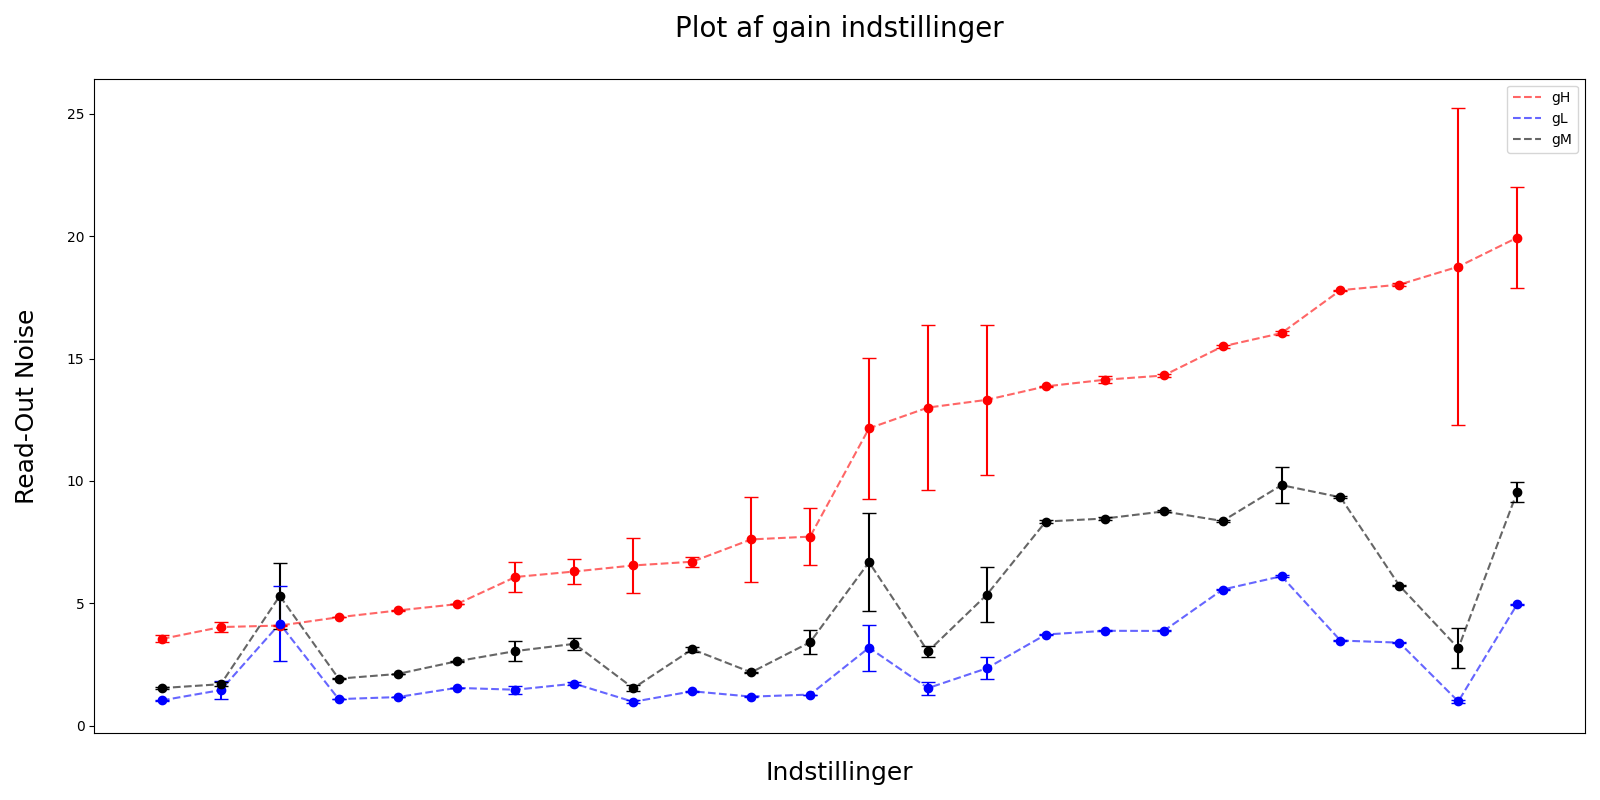
\includegraphics[width = \textwidth]{../Plots/gain.png}	
\end{figure}

\subsection{Read-out-rate-Indstilling}
Ved 'read-out rate' finde vi følgende forhold,
\[
r0.1 > r1 > r4
.\]
Read-out rate er et mål for kameraet udlæsningnshastighed. Altså et mål for hvor meget tid kameraet bruger på oversætte hver bin til en pixel på billedet. Det giver dermed fint mening at en høj read-out rate, og dermed langsom og omhyggelig udlæsning, giver den mindst mulige read-out noise
\begin{figure}[ht]
\centering
\sidecaption{Plot af read-out-rate}
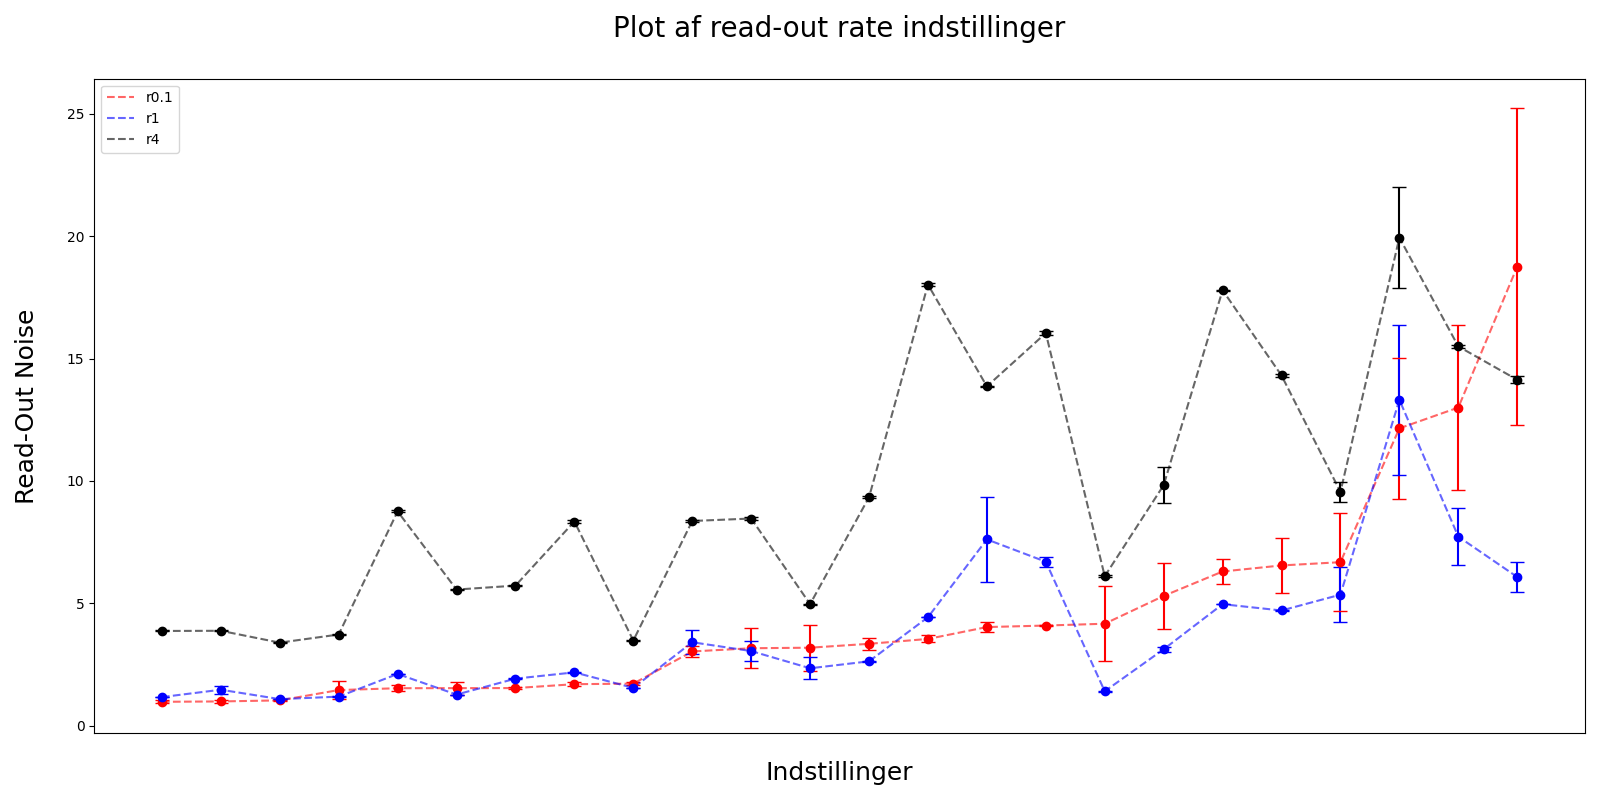
\includegraphics[width = \textwidth]{../Plots/read-out-rate.png}	

\end{figure}
\subsection{Bedste indstillinger}
Udover at kigge på, hvordan de enkelte indstillinger påvirker read-out noisen, så  vil vi også gerne kigge på, hvilket sæt af indstillinger der giver den mindste read-out noise. Det vil vi gøre, ved at lave et samlet plot med alle de målte read-out noises på. Vi vil så prøve at estimere, hvilket sæt af indstillinger der giver den laveste read-out noise. De 5 bedste punkter vil vi farvekode, så de adskiller sig fra de andre. Det kunne måske være, at der var en indstilling, der var mere følsom i forhold til at inducere read-out noise. 
\\
Efter analysen kan man måske gå ind og vurdere på hvilken indstilling der er mest følsom overfor read-out noise. 
\section{Dark Current og Noise}
\subsection{Er Dark Current konstant?}
Det første vi har overvejet, er hvorvidt Dark Current er uafhængig af indstillingen på CCD-kameraet. Vi undersøgte derfor Dark Current for hver eneste indstilling, og beregnede Dark Current tilvæksten for hver af disse. Vi fittede derefter alle disse punkter til en konstant, og overvejede hvorvidt dette fit var fornuftigt.
% \begin{marginfigure}
% 	Der skal lige defineres et enviroment til det her.
% \end{marginfigure}
\\
Fittet følger her,
\begin{figure}[ht]
	\centering
	\sidecaption{Fit af Dark Charge til en konstant funktion, usikkerheden er medtaget i linjen. Hvor errorbars ikke er synlige, er usikkerheden inkluderet i punktet.}
	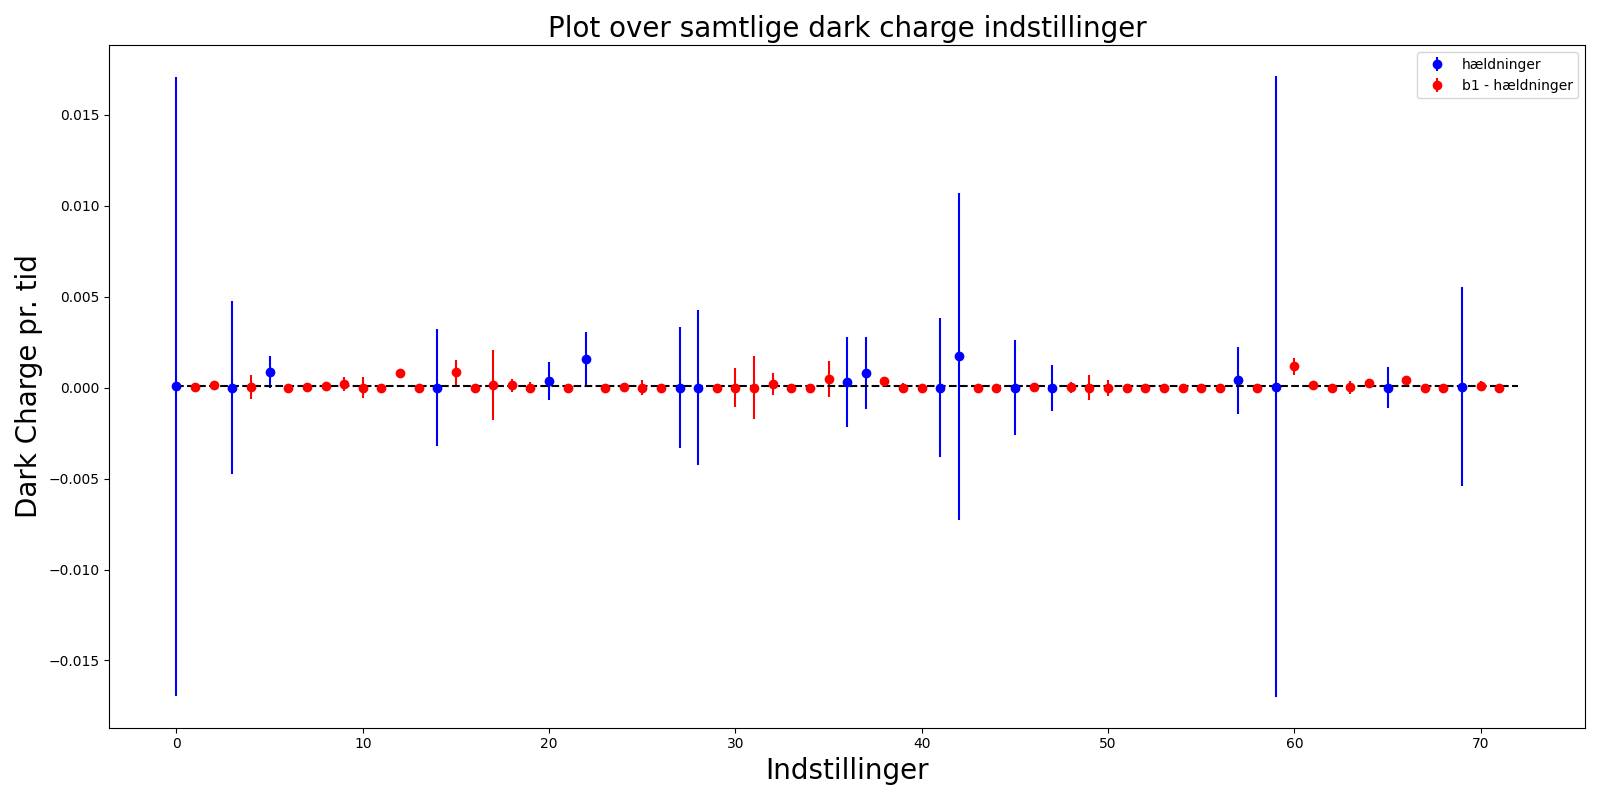
\includegraphics[width = \textwidth]{Plots/dark_hældninger_1.png}
\end{figure}
\\
Her er alle punkter medtaget, men punkterne med indstillingen \textbf{b1} er markeret med blå, da denne indstilling generelt gav en større usikkerhed. Vi undersøgte derfor hvordan fittet så ud når, disse indstillinger blev udelukket.
\begin{figure}[ht]
	\centering
	\sidecaption{Fit af Dark Charge, hvor indstilingen \textbf{b1} ikke er inkluderet.}
	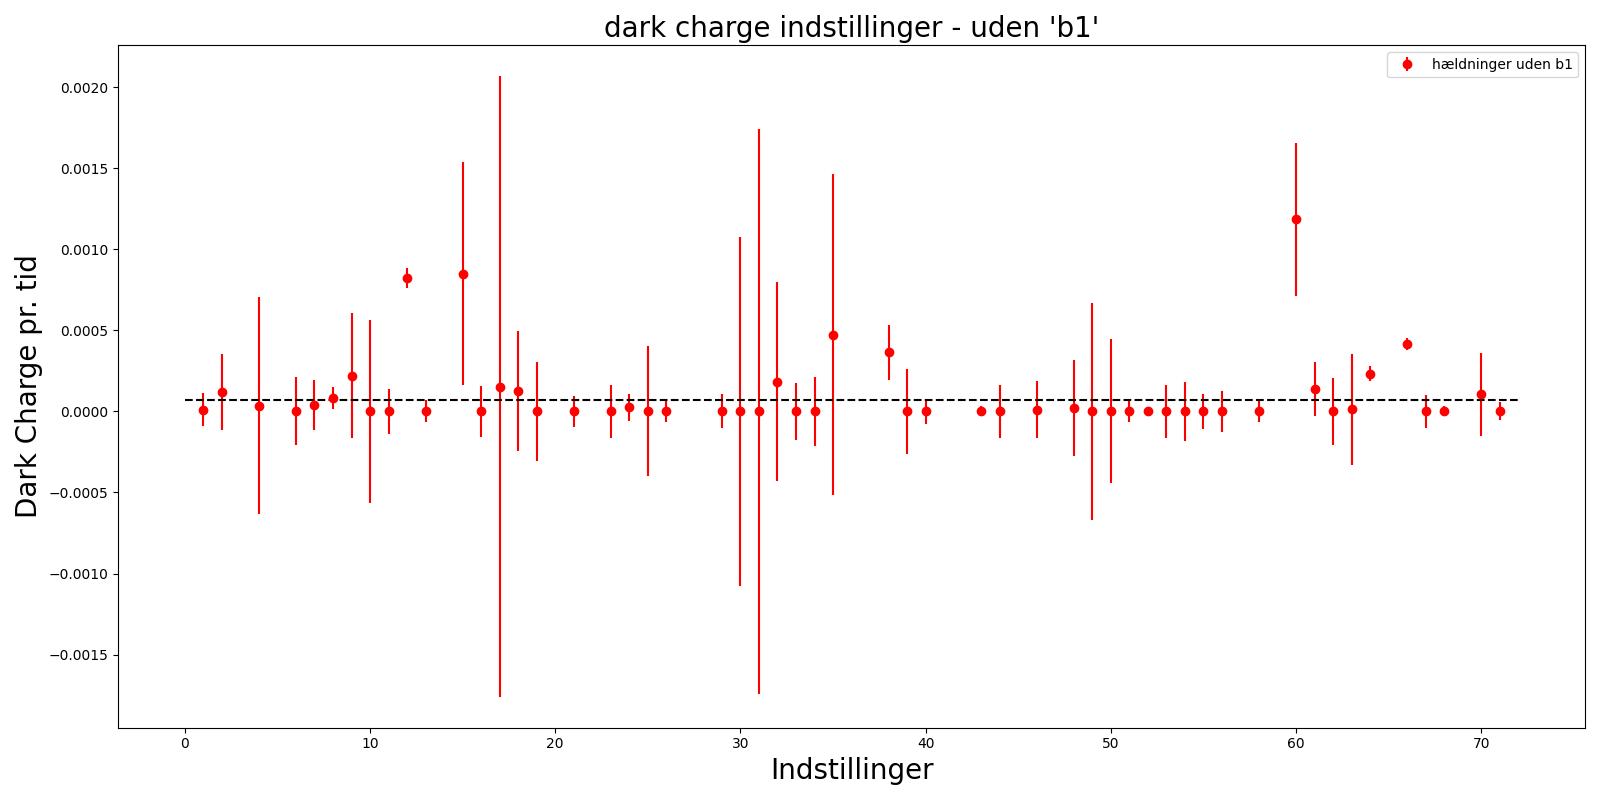
\includegraphics[width = \textwidth]{Plots/dark_hældninger_2.png}
\end{figure}
\\ 
I begge tilfælde ser fittet ganske fornuftigt ud, men det er tydeligt at \textbf{b1} indstillingen giver anledning til de største usikkerhed. Vi konkluderer at Dark Current er konstant på tværs af indstillinger.
\section{Vurdering af kamera}
Efter analysen af ens data, kan man måske gå ind og vurdere på, om kameraet er godt nok til det forsøg, som man skal lave med det. Men det er ikke helt meningen med den her rapport
\printbibliography
\end{document}
